%%%%%%%%%%%%%%%%%%%%%%%%%%%%%%%%%%%%%%%%
% PDF compatibility code. 

\makeatletter
\newif\ifpdflatex@
\ifx\pdftexversion\@undefined
\pdflatex@false
%\message{Not using pdf}
\else
\pdflatex@true
%\message{Using pdf}
\fi

\newcommand{\latexorpdf}[2]{
  \ifpdflatex@ #2
  \else #1
  \fi
}

\makeatother

#ifdef A4Format
\newcommand{\pformat}{a4paper}
#endif A4Format
#ifdef LetterFormat
\newcommand{\pformat}{letterpaper}
#endif LetterFormat

%%%%%%%%%%%%%%%%%%%%%%%%%%%%%%%%%%%%%%%%

\latexorpdf{
\documentclass[\pformat,12pt,twoside]{article}
}{
% pdftex option is used by graphic[sx],hyperref,toolbox.sty
\documentclass[\pformat,pdftex,12pt]{article}
}

% Ueki change
%\newcommand{\vdmtools}{\textbf{VDMTools}$^{\mathbf{{\textregistered}}}$}
\newcommand{\vdmtools}{\textbf{VDMTools}}
% Ueki change

\newcounter{guideno}
\setcounter{guideno}{1}
\newcommand{\guideline}[1]{%
  \fbox{\parbox{.98\textwidth}{{\bf Guideline \theguideno:} #1
        \addtocounter{guideno}{1}}}}

\usepackage{color}
\usepackage{colortbl}

\newcolumntype{G}{>{\columncolor[gray]{0.8}}p{.9\textwidth}}
\newenvironment{VDMgray}%
{\begin{tabular}{|G|}\hline\small\begin{alltt}}%
{\end{alltt}\normalsize\\
 \hline\end{tabular}}

\setcounter{topnumber}{3}
\def\topfraction{1.0}
\setcounter{bottomnumber}{3}
\def\bottomfraction{1.0}
\setcounter{totalnumber}{3}
\def\textfraction{.1}

\usepackage{times}
\usepackage{longtable,multirow}

% Ueki change start
\usepackage[dvipdfm,bookmarks=true,bookmarksnumbered=true,colorlinks,plainpages=true]{hyperref}
\usepackage{cite}

\def\seename{$\Rightarrow$}
% Ueki change end

% Ueki delete start
%\latexorpdf{
%\usepackage[plainpages=true,colorlinks,linkcolor=black,citecolor=black,pagecolor=black, urlcolor=black]{hyperref}
%}{
%\usepackage[plainpages=true,colorlinks]{hyperref}
%}
% Ueki delete end

\usepackage{toolbox}
\usepackage{vdmsl-2e}
\usepackage{makeidx}
\usepackage{alltt}
\usepackage{here}

\usepackage{longtable}
\usepackage{ifthen}
% plainpages=false: avoid warning
%   destination with the same identifier already exists
%   but it do not seem to work a the first pages

\usepackage{vpp}

%\renewcommand{\vdmpp}{{\small VDM}$^{++}$}

\makeatletter
% ------------- TOC manipulation ------------
\def\docglbldepth{1}
%\setcounter{secnumdepth}{\docglbldepth}
%\setcounter{tocdepth}{\docglbldepth}
\def\@pnumwidth{3.0em}
% more space for for >10 subsections
%\def\l@section{\@dottedtocline{1}{1.5em}{3.1em}}
\def\l@subsection{\@dottedtocline{2}{1.5em}{2.8em}}
%\def\l@subsubsection{\@dottedtocline{3}{4.3em}{3.6em}}
%\def\l@paragraph{\@dottedtocline{4}{7.9em}{4.1em}}
%\def\l@subparagraph{\@dottedtocline{5}{10em}{5em}}
\makeatother

\begin{document}

\vdmtoolsmanualscsk{VDM++ Method Guidelines}{2.0}



% No line numbering
\nolinenumbering
\setindent{outer}{\parindent}
\setindent{inner}{0.0em}

\newcommand{\tab}{\makebox[4em]{}}

\definecolor{color1}{rgb}{0.000,0.000,0.000}
\definecolor{color2}{rgb}{0.000,0.000,1.000}
\definecolor{color3}{rgb}{0.000,1.000,1.000}
\definecolor{color4}{rgb}{0.000,1.000,0.000}
\definecolor{color5}{rgb}{1.000,0.000,1.000}
\definecolor{color6}{gray}{0.5}
%{rgb}{1.000,0.000,0.000}
%\definecolor{not_covered}{gray}{0.5}   %gray for previewing
\definecolor{color7}{rgb}{1.000,1.000,0.000}
\definecolor{color8}{rgb}{1.000,1.000,1.000}
\definecolor{color9}{rgb}{0.000,0.000,0.502}
\definecolor{color10}{rgb}{0.000,0.502,0.502}
\definecolor{color11}{rgb}{0.000,0.502,0.000}
\definecolor{color12}{rgb}{0.502,0.000,0.502}
\definecolor{color13}{rgb}{0.502,0.000,0.000}
\definecolor{color14}{rgb}{0.502,0.502,0.000}
\definecolor{color15}{rgb}{0.502,0.502,0.502}
\definecolor{color16}{gray}{0.5}
%{rgb}{1.000,0.000,0.000}
%\definecolor{not_covered}{gray}{0.5}   %gray for previewing
%\definecolor{color16}{rgb}{0.753,0.753,0.753}

\vfill
\begin{abstract}
The limitations of graphical models in object-oriented analysis 
are widely accepted. While superior for visualization, a graphical 
model is not enough for precise and unambiguous specification. 

This document presents a methodology and tools that combine the 
benefits of graphical modeling in UML with a pragmatic and light-weight 
approach to formal modeling and validation in the object-oriented 
formal specification language VDM++, supported by \vdmtools.

\vdmtools\ provides round trip engineering between VDM++ and UML 
(Rational Rose). In this way, a user of UML gets access to enhanced 
analysis and validation facilities such as type checking and 
testing of executable models with automatic checking of annotations 
such as invariants and pre- and post-conditions. 
\end{abstract}
\vfill

\newpage

\section{Introduction}

In object-oriented modeling the use of graphical visualization 
can help to master complexity and significantly increase the 
understanding of the ``problem'' being modeled. Graphical diagrams 
can give an abstract and high-level overview of a model, which, 
for example, can be of great value for analyzing requirements 
in the early phases of the software process. In the later phases, 
the diagrams can improve the documentation of the code, again 
by aiding general understanding.

Graphical models for analysis are suitable both for a software 
engineer and a client with no programming background. However, 
it happens that people have different perceptions of what a graphical 
model actually says. This lack of common understanding can be 
due to the complexity of a model, but even for small models it 
can be difficult to assess and review a model, and predict the 
exact consequences of the boxes and arrows that it contains. 

In contrast, executable models are suitable for automating the 
assessment of models, allowing models to be validated early in 
the software development process. Combined with rapid prototyping 
capabilities for designing graphical front-ends, executable models 
can greatly reduce the incidence and severity of late rework 
so that products can be delivered on schedule and within budget. 
For example, by executing a model the engineer can get immediate 
feedback on his specification. And by extending a model with 
a graphical front-end matching the problem domain and activities 
of a client, the client can get a clear view of the specifier's 
understanding of the requirements by interacting directly with 
the model via the front-end.

This document presents a methodology and tools to enhance
object-oriented analysis and design by combining the benefits of
graphical modelling in UML with those of executable models in the
object-oriented formal specification language VDM++\footnote{{\small
VDM++ is an object-oriented extension of ISO Standard VDM-SL. Standard
VDM-SL does not provide a structuring mechanism, though VDM-SL
supports modules.  VDM++ supports UML-like classes and other OO
concepts}.}.  Formal specification can improve the modelling process by
adding precision while keeping abstraction. Without precision it would
not be possible to automate any parts of the validation
process. Abstraction is vital in order to focus on the conceptual
properties rather than their detailed and complex implementation. In
addition to stating requirements in an unambiguous and structured way,
precise models can be analysed and validated automatically using tools
and techniques familiar to engineers, such as testing and rapid
prototyping. IFAD calls its approach ``Validated Design through
Modelling'' (VDM), which is supported by \vdmtools. The document
assumes that readers already have some familarity with general
object-oriented software development \cite{Meyer88,Shlaer88,Rumbaugh&91}.

\subsection{VDM++ and UML}

Roughly speaking, no two companies develop software in the same 
way. Even within one company the software process can vary among 
projects and people. In principle, VDM can be used as an add-on 
to improve any software process, whether object-oriented (using 
VDM++), structural (using VDM-SL) or ad-hoc (using either one). 
However, in this document, we focus on how UML and VDM++ can 
be used together. Moreover, we shall focus on how to construct 
a model without distinguishing between the typical phases of 
software processes such as requirements analysis and system design. 
This is because the main difference between the phases lies in 
the level of abstraction. The basic approach to constructing 
models and analysing them using \vdmtools\ is the same.

In order to provide users with the complementary benefits of 
UML and VDM++, the VDM++ Toolbox, which is one toolset of \vdmtools, 
offers the Rose-VDM++ Link \cite{UMLMan-SCSK}. This facilitates an easy transition 
between UML and VDM++ models. It translates UML class diagrams 
automatically to VDM++ specifications, and vice versa, providing 
full round-trip engineering capabilities. Other aspects of UML 
like use cases can be employed independently of the VDM++ model. 
Typically use cases will precede a VDM development. Roughly speaking, 
a VDM++ model is really a textual, precise version of UML class 
diagrams incorporating all the details that are often missing 
or described vaguely using natural language there. Hence, the 
UML and VDM++ models are complementary and, in fact, can be seen 
as two views of the same model. 

In the more recent versions of UML there is a notation called OCL
(Object Constraint Language) which has many similarities with VDM++,
e.g.\ pre- and post-conditions. However VDM++ is preferable to OCL
because \vdmtools\ enables validation based on testing
principles. This can never be possible for OCL because it contains no
executable subset.

This document does not provide complete introductions to UML, 
VDM++ nor the VDM++ Toolbox. For further information the reader 
can consult \cite{Booch&99,LangManPP-SCSK,UserManPP-SCSK}.

\subsection{Constructing a Model}

The way a model is constructed is not only dependent on the choice 
of notation. The purpose of the model is of vital importance 
as well and is determined by the kind of analysis to be conducted. 
When designing a car, the purpose of one model may be to test 
the aerodynamics, the purpose of another to test the brake system, 
the purpose of a third to test the injection system, and so on. 
Each of these models can abstract away from aspects of the other 
models. For example, the models of the brake and injection systems 
can be analysed separately. The abstraction determines which 
details will be represented and which will be ignored because 
they are not relevant to the analysis. Abstraction is the tool 
to cope with complexity of the systems under construction.

After establishing the purpose of a model, the following list 
of steps can be a helpful guide to its construction:

\begin{enumerate}
\item Read the requirements.
\item Analyse the functional behaviour from the requirements.
\item Extract a list of possible classes or data types (often from 
nouns) and operations (often from actions). Create a directory 
by giving explanations to items in the list.
\item Sketch out representations for the classes using UML. This includes 
the attributes and the associations between classes. Check the 
internal consistency of the model in VDM++.
\item 
Sketch out signatures for the operations. Check the model's consistency 
in VDM++.
\item Complete the class (and data type) definitions by determining 
potential invariant properties from the requirements and formalising 
these.
\item Complete the operation definitions by determining pre- and post-conditions 
and operation bodies, modifying the type definitions if necessary.
\item Validate the specification using testing and rapid prototyping.
\item Implement the model using automatic code generation or manual 
coding.
\end{enumerate}

Step 2 could either be dealt with using traditional use cases from UML
or by making a few VDM definitions without any structuring. Most
newcomers to VDM++ are probably going to make use cases but an
example of the other approach is given in \cite{CashPoint}.
Roughly speaking step 1 to 5 above are the parts that are carried 
out in a conventional object-oriented UML design. The only difference 
is that the VDM++ coupling is able to find more inconsistencies 
in step 4 and 5. However, as we will see later the remaining 
steps (6 to 8) are able to identify quite subtle and important 
design considerations that must be dealt with to ensure the integrity 
of the system.

In the following section we present the requirements for a simple 
alarm and expert scheduling system for a chemical plant. This 
is modelled in the rest of the document. Though the modelling 
process is described as a one-pass process in this document, 
a real development would usually be an iterative process. Furthermore,
since the example used for illustration purpose here is so
small we will omit step 2 from the list given above.

\section{A Chemical Plant Example}

This section presents the requirements for a simple alarm system 
of a chemical plant. The example is inspired by a subcomponent 
of a large alarm system developed by IFAD and was introduced 
in the VDM-SL book by Fitzgerald and Larsen \cite{Fitzgerald&98b}. 
We will develop and validate a model of the system using the 
facilities of the VDM++ Toolbox, including the Rose-VDM++ Link.

A chemical plant is equipped with a number of sensors that are 
able to raise alarms in response to conditions in the plant. 
When an alarm is raised, an expert must be called to the scene. 
Experts have different qualifications for coping with different 
kinds of alarm. The individual requirements are labelled R1-R8 
for reference.

\begin{description}
\item[R1] A computer-based system is to be developed to manage the alarms 
of this plant.
\item[R2] Four kinds of qualification are needed to cope with the alarms. 
These are electrical, mechanical, biological, and chemical.
\item[R3] There must be experts on duty during all periods allocated in 
the system.
\item[R4] Each expert can have a list of qualifications.
\item[R5] Each alarm reported to the system has a qualification associated 
with it along with a description of the alarm that can be understood 
by the expert.
\item[R6] Whenever an alarm is received by the system an expert with the 
right qualification should be found so that he or she can be 
paged.
\item[R7] The experts should be able to use the system database to check 
when they will be on duty.
\item[R8] It must be possible to assess the number of experts on duty.
\end{description}

In the next section we start the development of a model of an 
alarm system to meet these requirements.

\section{Graphical Model in UML}

We shall now develop our first model of the alarm system described 
above. The purpose of the model is to clarify the rules governing 
the duty roster and calling out of experts to deal with alarms. 
We construct a model in UML and use \vdmtools\ to check its consistency. 
Whenever we wish to emphasise a methodological guideline specific 
to the UML/VDM++ combination we will highlight it by a small 
statement. 

\subsection{Creating a Directory}

Following the guidelines for constructing a model, we first extract 
a list of possible classes and data types:

\textbf{Potential classes and types (nouns)}
\begin{itemize}
\item Alarm: required qualification and description
\item Plant
\item Qualification (electrical, mechanical, biological, chemical)
\item Expert: list of qualifications
\item Period 
\item System and system database? Probably this is a kind of schedule.
\end{itemize}

Using a UML tool such as Rational Rose this part of the directory 
would often be modelled in a class diagram; this is what is done 
in the next step in the guide. However, if the system to be designed 
is large it may be safer to systematically list all the potential 
classes and types in a directory as shown here.

\textbf{Potential operations (actions)}
\begin{itemize}
\item Expert to page: given alarm (involved: alarm operator and system)
\item Expert is on duty: check when on duty (involved: expert and system)
\item Number of experts on duty: given period presumably (involved: 
operator? and system)
\end{itemize}

Using a UML tool this part of the directory would often be described 
as use cases.

For this simple system we will let the above lists work as a 
dictionary of the main concepts in the system, though better 
explanations would be appropriate.

\subsection{Sketching Class Representations}

Having created a directory it is now necessary to explain what 
the difference is between a class and a type. In pure OO approaches 
there is no distinction and this has the consequence that one 
often gets a very large collection of classes and can therefore 
have difficulties in mastering the complexity due to the number 
of classes. In VDM++ there is a distinction between classes and 
types and we wish to use this to reduce the number of classes 
for our model. Generally speaking types correspond to what is 
known as container classes in conventional OO approaches. These 
are classes that simply have a number of attributes which users 
of the class can read and write. 


\guideline{Nouns from a directory should be modelled as 
types if they have no ``real'' functionality (in addition to read/write) 
with respect to the purpose of the model.}


Qualification from the dictionary above is an example of a noun 
that is better modelled as a type. Qualification is an enumeration 
type since it holds just four possible values and has no obvious 
functionality. If the purpose of our model included the different 
kinds of actions different experts could carry out depending 
upon their qualification, it would have been more natural to 
model qualification as a class.

Let us now consider alarm and expert from the dictionary. Both 
of these correspond to groupings of real objects in the physical 
world of our example, which co-exist and act independently. We 
will therefore model both of these as classes:

\begin{description}
\item[Alarm] is a class with attributes \textit{required qualification} 
and \textit{description}. Description is a string that can be considered 
a type in the same way as \textit{Qualification} (see Figure~\ref{fig:alarm}).

\begin{figure}[htbp]
\begin{center}

\includegraphics[width=1.833in]{alarm}
\caption{The Alarm Class.\label{fig:alarm}}
\end{center}
\end{figure}

\item[Expert] is a class with \textit{qualifications} as an attribute. 
The requirements state that there is a list of qualifications. 
The word list implicitly implies some kind of ordering but we 
do not know from the requirements anything about how this ordering 
should be. We need to have this clarified with our ``customer'', 
but for the time being we will assume that there is no specific 
ordering which has importance for the desired functionality. This is
shown in Figure~\ref{fig:expert}.
\end{description}

\begin{figure}[htbp]
\begin{center}
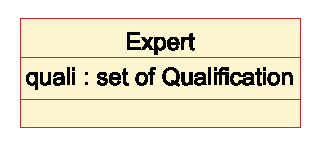
\includegraphics[width=1.833in, height=0.714in]{expert}
\caption{The Expert Class.\label{fig:expert}}
\end{center}
\end{figure}

Somehow we need to make some connection to associate alarms and 
a schedule of experts. In order to be able to express the \textit{precise 
limitations} in the UML/VDM++ methodology for such connections 
we typically recommend creating a main class, containing associations 
to the other classes. 


\guideline{Create a ``main'' class to represent the entire 
system such that the precise limitations between the different 
classes and their associations can be expressed here.}


In our example the main class will be \textbf{Plant}. Recall that 
the purpose of our model is to clarify the rules concerning the 
duty schedule and the calling out of experts to deal with alarms. 
We choose Plant as a class to model an abstract perspective focusing 
on this purpose. Hence, two aspects of the ``plant'' are important: 
the \textit{schedule} of experts on duty and the collection of (registered) 
possible \textit{alarms}. Let us consider the alarms first. We need 
to have an association from the Plant class to the Alarm class 
and since we may have more than one alarm in our system we need 
to use a multiplicity with this association. We call this association \textit{alarms} 
(see figure below).


\guideline{Whenever an association is introduced one should 
consider the multiplicity of it and give it a role name in the 
direction in which one wishes to use the association.}


Let us now consider the schedule that must hold a number of experts 
allocated to periods. For each period we can have zero or more 
experts on duty. Thus we need to use an association which is 
qualified with period and has a multiplicity of zero or more. 
We call this association \textit{schedule}.


\guideline{If an association depends on some value a qualifier 
should be introduced for the association. The name of the qualifier 
must be a VDM++ type.}


We are not told much about periods in the requirements, and we 
don't need to know much with the chosen focus of the model. We 
can model period as a type because it does not contain any ``real'' 
functionality. 

At this point in time the class diagram for our system can be 
drawn with three classes as shown in Figure~\ref{fig:firstclassdia}.
\begin{figure}[htbp]
\begin{center}
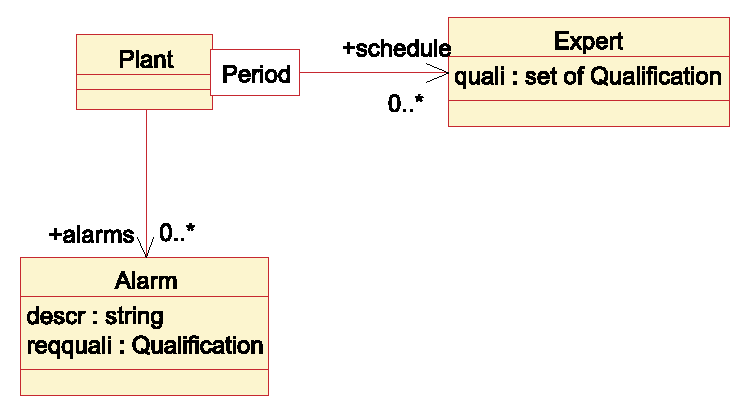
\includegraphics[width=4in]{firstclassdia}
\caption{Initial Class Diagram.\label{fig:firstclassdia}}
\end{center}
\end{figure}

Here we have used Rose, adding attributes and establishing relationships 
between the classes. We enter attributes and their types according 
to the templates provided by Rose. The types are VDM++ types, 
e.g. the set type constructor ``set of'' and class names and other 
type identifiers. All of this could equally well have been done 
directly in VDM++, and sometimes developers find it faster to 
write the textual model first and produce the graphical visualization 
using the Rose-VDM++ Link.

There is no such thing as the right model. For example, if we 
wanted to clarify the business processes concerning the use of 
this alarm subsystem, perhaps as part of a larger computer system, 
then our model would probably be different. We might want to 
focus more on how schedules are constructed and maintained.

Next we map the UML model to VDM++ skeletons automatically, using 
the Rose-VDM++ Link. These are included below.

\subsubsection*{The class Plant}

\begin{VDMgray}
--
-- THIS FILE IS AUTOMATICALLY GENERATED!!
--
-- Generated at Mon 09-Aug-99 by the Rose VDM++ Link
--
class Plant

instance variables
 alarms : set of Alarm;
 schedule : map Period to set of Expert;

end Plant
\end{VDMgray}

Note that \emph{schedule}, which is a qualified association in UML, 
is translated to a mapping in VDM++. A mapping is like a table, 
where it is possible to look up with a key (in the domain) to 
get the associated value (in the range). Above, the key is a 
period and the value is a set of experts. Also note that the 
VDM++ set type is used to represent unordered ``zero-or-many'' 
associations, as in the \emph{alarms} instance variable.

\subsubsection*{The class Expert}

\begin{VDMgray}
--
-- THIS FILE IS AUTOMATICALLY GENERATED!!
--
-- Generated at Mon 09-Aug-99 by the Rose VDM++ Link
--
class Expert

instance variables
 quali : set of Qualification;

end Expert
\end{VDMgray}

Note again that the VDM++ set type is used to represent the UML 
association with a ``zero-or-many'' multiplicity for the \emph{quali}
instance variable.

\subsubsection*{The class Alarm}

\begin{VDMgray}
--
-- THIS FILE IS AUTOMATICALLY GENERATED!!
--
-- Generated at Mon 09-Aug-99 by the Rose VDM++ Link
--
class Alarm

instance variables
 descr : string;
 reqquali : Qualification;

end Alarm
\end{VDMgray}

Note that attributes of UML classes become instance variables 
of VDM++ classes, just like UML associations. The difference 
is that the type of an attribute is not a class.

\subsubsection*{Type checking the classes}


\guideline{Use \vdmtools\ to check internal consistency as soon as
class skeletons have been completed (before any functionality 
has been introduced).}


Using \vdmtools\ we can try to type check the model in order to 
ensure its internal consistency, i.e. that all identifiers are 
well-defined. The three classes above are not type correct, as 
there are three identifiers that are not defined: \emph{Period},
\emph{Qualification} 
and \emph{string} (not built-in in VDM++). Therefore the following three 
type definitions are inserted into the three VDM++ classes respectively.

\begin{VDMgray}
class Plant

types
 public Period = token;

instance variables 
...
end Plant
\end{VDMgray}

The type \emph{token} contains an infinite set of unspecified values 
with equality as the only operator. It is used because we do 
not care what representation for periods that will be chosen 
in the final implementation at this point of time. We abstract 
away from this. The type \emph{Period} needs to be declared
\texttt{public} because it must be available outside the \emph{Plant} class.

\begin{VDMgray}
class Expert

types
 
 public Qualification = \texttt{<}Mech\texttt{>} {\textbar} \texttt{<}Chem\texttt{>} {\textbar} \texttt{<}Bio\texttt{>} {\textbar} \texttt{<}Elec\texttt{>};

instance variables 
...
end Expert
\end{VDMgray}


Qualification is an enumeration type defined as unions (vertical 
bars) of quote types in VDM++. A quote type has the same name 
as the single value that it holds, which must be written in ``\texttt{<}'' 
and ``\texttt{>}'' signs.

\begin{VDMgray}
class Alarm

types
 public string = seq of char;

instance variables 
 descr : string;
 reqquali : Expert\`{}Qualification;

end Alarm
\end{VDMgray}


Note that the type of the instance variable \emph{reqquali} has been
prefixed with the class name \emph{Expert} since \emph{Qualification}
is defined there. Using the Rose-VDM++ Link, this change is updated at
the Rose UML level automatically as shown in Figure~\ref{fig:updatedalarm}.

\begin{figure}[htbp]
\begin{center}
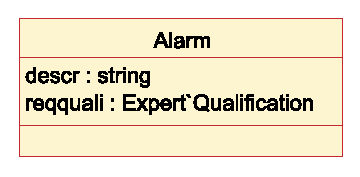
\includegraphics[width=2.120in]{updatedalarm}
\caption{The Updated Alarm Class.\label{fig:updatedalarm}}
\end{center}
\end{figure}

The type definitions do not have a counter part in the UML model 
and are therefore not translated. However they are kept in the 
VDM++ model files and cannot be deleted (or changed) by updates 
in the UML model.

\subsection{Sketching Signatures for operations}

We continue the development by adding operation signatures in 
UML. All three operations listed in the directory above belong 
naturally in the class Plant, because they are dependent on the 
schedule which is allocated there.
The updated class diagrams for Plant is shown in Figure~\ref{fig:updatedplant}.

\begin{figure}[htbp]
\begin{center}

\includegraphics[width=3in]{updatedplant}
\caption{The Updated Plant Class.\label{fig:updatedplant}}
\end{center}
\end{figure}

The signatures of the operations are straightforward. For example, 
the \textit{ExpertToPage} operation takes an alarm and a period as input 
and returns an expert as a result. 


\guideline{Think carefully about the parameter types and 
the result type as this activity often is able to identify missing 
connections in the class diagram.}


The updated skeleton VDM++ class is produced automatically.

\begin{VDMgray}
class Plant

types
 public Period = token;

instance variables
 alarms : set of Alarm;
 schedule : map Period to set of Expert;

operations
 ExpertToPage : Alarm * Period ==\texttt{>} Expert
 ExpertToPage(a, p) ==
   is not yet specified;

 ExpertIsOnDuty : Expert ==\texttt{>} set of Period
 ExpertIsOnDuty(ex) ==
   is not yet specified;

 NumberOfExperts : Period ==\texttt{>} nat
 NumberOfExperts(p) ==
   is not yet specified;

end Plant
\end{VDMgray}


It is possible to syntax and type check the model we have developed 
above but it is too vague to be of much use for validation purposes. 
Our next step is to add more precision to this model using VDM++. 
Note that traditionally most UML developers would stop at this 
step and as we shall see below the most important analysis and 
design discoveries are still to come.

\section{Making the Model More Precise}

At this stage it is a good idea to review the requirements to 
see that our model covers the individual ones satisfactorily. 
Clearly we have not yet considered the operations in detail, 
so \textbf{R6}---\textbf{R8} are not fully covered. Otherwise the requirements seem 
covered reasonably well, except that we have not documented requirement 
\textbf{R3} anywhere:

\begin{description}
\item[R3] There must be experts on duty during all periods 
allocated in the system.
\end{description}

However, the graphical and the type checked VDM++ model above 
has some further hidden assumptions and unclear aspects as we 
shall see below.

Typically a person implementing a model will not, and should 
not, do this from the original requirements directly, but using 
analysis and design models with accompanying comments. That is 
one purpose of models. Hence, the more precise, yet abstract, 
we can make such models the lower is the risk of an erroneous 
implementation, without prejudice to choice of implementation.

\subsection{Adding Invariant Properties}

We can formulate requirement \textbf{R3} in a precise way in the VDM++ 
model. First, what does it mean that a period is allocated in 
the system? This is when it is in the schedule for experts on 
duty, i.e.\ in the domain of the instance variable schedule, which 
is a mapping from periods to sets of experts. 

\begin{VDMgray}
 forall p in set dom schedule \& 
   \textit{there are experts on duty in p}
\end{VDMgray}

Next, what does it mean that there are experts on duty for a 
period? It means that the range value associated with the period, 
namely a set of experts, is non-empty. 

\begin{VDMgray}
 forall p in set dom schedule \& schedule(p) \texttt{<}\texttt{>} \{\};
\end{VDMgray}


In VDM++, this predicate is added as an invariant (abbreviated \texttt{inv}) 
in the instance variables section of the class \emph{Plant}:

\begin{VDMgray}
class Plant
...

instance variables
 alarms : set of Alarm;
 schedule : map Period to set of Expert;
 inv 
   forall p in set dom schedule \& schedule(p) \texttt{<}\texttt{>} \{\};

...
end Plant
\end{VDMgray}


An invariant is a condition that must hold always of an object 
state.

\guideline{You should try to document important properties 
or limitations as invariants because some part of a system may 
implicitly assume some invariant property to hold that other 
parts should be aware of.}

\subsection{Completing Operation Definitions}

Next we consider conditions associated with operations, pre-conditions 
and post-conditions respectively. A pre-condition formalises 
assumptions made by an operation, i.e. what must hold of the 
parameters and object state before an operation is executed. 
A post-condition states what an operation provides, i.e. what 
holds after it has been executed. Thus the post-condition is 
a relation between the initial object state and parameters on 
one side, and the final state and the result on the other. For 
example, the operation \emph{ExpertToPage} takes an alarm and a period 
as inputs and returns an expert to handle the alarm. Will it 
accept an arbitrary alarm or period (pre-condition)? And what 
must hold of the expert (post-condition)?

\texttt{ExpertToPage} has the following signature:

\begin{VDMgray}
 ExpertToPage : Alarm * Period ==\texttt{>} Expert
\end{VDMgray}

However, as indicated above, it cannot treat any alarm and period. 
First, the period must be known about in the schedule, in order 
to ensure that there are experts on duty. It also seems obvious 
to require that the alarm has been registered in the system, 
i.e. that it is among the possible alarms contained in the instance 
variable alarms:

\begin{VDMgray}
 ExpertToPage : Alarm * Period ==\texttt{>} Expert
 ExpertToPage(a, p) ==
   is not yet specified
 pre a in set alarms and
     p in set dom schedule
\end{VDMgray}

Moreover, the operation should not return any expert on duty. 
The expert should have the right qualification to cope with the 
alarm. This is documented in the post-condition:

\begin{VDMgray}
 post let ex = RESULT in
        ex in set schedule(p) and
        a.GetReqquali() in set ex.GetQuali();
\end{VDMgray}

The let-expression just binds the result of the operation to an
identifier. The first conjunct says that the result expert is on duty,
the second that the qualification requirement is met. Here we have
assumed that access operations \texttt{GetReqquali} and
\texttt{GetQuali} are defined for the \texttt{Alarm} and
\texttt{Expert} classes respectively.  Because of information exchange
these kind of access operations must often be defined in OO
developments, but they are trivial to define. We do not need to
specify a body of the operation at this stage, but this is introduced
later in order to make the operation executable.

Note that the definition given here does not state which of the 
experts should be chosen if more than one expert with the right 
qualification is on duty in the given period. The requirements 
have not given us any way to see what the most desirable choice 
is and therefore this implicit definition leaves freedom to decide 
on this issue later in the development process.


\guideline{When several choices are possible you should try to use
implicit ways of describing the desired functionality.}


Now we can ask ourselves whether it is always possible to return 
such an expert with the right qualification? We cannot be sure 
in the current model as there is no limitation on the schedule of 
experts on duty in relation to the registered alarms. However, 
we can introduce this dependency by adding an invariant property:

\begin{VDMgray}
instance variables
 alarms : set of Alarm;
 schedule : map Period to set of Expert;
 inv forall p in set dom schedule \& schedule(p) \texttt{<}\texttt{>} \{\};
 inv forall a in set alarms \&
        forall p in set dom schedule \&
           exists ex in set schedule(p) \&
              a.GetReqquali() in set ex.GetQuali();
\end{VDMgray}

The new invariant says that for any alarms and periods registered 
in the system there must be an expert on duty in the period who 
has the right qualification to handle the alarm. This ensures 
that the specification of \texttt{ExpertToPage} makes sense and is implementable, 
i.e. a desired expert can always be found. Note that because 
of the precision of the VDM++ model we have been forced to ask 
ourselves such detailed questions related to the desired functionality 
of the system. For example, the above invariant would also be 
important if the system was extended to support that experts 
could change their shifts. The invariant identifies a property 
which is a dominant design parameter for the system, but which 
is not identified using the conventional OO approach. 


\guideline{You should try to identify additional invariant 
properties when operations are being described.}


\texttt{NumberOfExperts} has the following signature:

\begin{VDMgray}
 NumberOfExperts : Period ==\texttt{>} nat
\end{VDMgray}

It must return the number of experts on duty in a given period. 
Probably we want the period to be a known one in the schedule. 
This is the pre-condition. The result should just be the cardinality 
of the set of experts on duty in the period. This is the body 
of the operation:

\begin{VDMgray}
 NumberOfExperts : Period ==\texttt{>} nat
 NumberOfExperts(p) ==
   return card schedule(p)
 pre p in set dom schedule;
\end{VDMgray}


We do not need a post-condition in this case, as it would just 
copy the body, which is already described in a fairly high-level 
way.

\texttt{ExpertIsOnDuty} has the following signature:

\begin{VDMgray}
 ExpertIsOnDuty : Expert ==\texttt{>} set of Period
\end{VDMgray}

It must be possible to ask when any expert is on duty so we do 
not need to specify a pre-condition for this operation. Again 
a post-condition is not necessary because the body of the operation 
can be described in a high-level and natural way:

\begin{VDMgray}
 ExpertIsOnDuty : Expert ==\texttt{>} set of Period
 ExpertIsOnDuty(ex) ==
   return \{p {\textbar} p in set dom schedule \& 
              ex in set schedule(p)\};
\end{VDMgray}

The body returns the set of periods in the domain of the schedule 
such that the given expert is on duty in the periods. Precise, 
clear and yet abstract! Such a statement could take up several 
lines of code in a programming language. In Java this would look something 
like: 

\begin{VDMgray}
import java.util.*;

class Alarm \{

  Map schedule;

    Set ExpertIsOnDuty(Integer ex) \{
      TreeSet resset = new TreeSet();
      Set keys = schedule.keySet();
      Iterator iterator = keys.iterator();

      while(iterator.hasNext()) \{
        Object p = iterator.next();
        if ( ( (Set) schedule.get(p)).contains(ex))
            resset.add(p);
      \}

      return resset;
   \}
\}
\end{VDMgray}


\guideline{Try to make explicit operation definitions 
in VDM++ precise and clear, and yet abstract compared to code 
written in a programming language.}

To summarise, let us map our changes in the (type checked and 
consistent) VDM++ model to the UML model, using the Rose-VDM++ 
Link. The resulting diagram is:

\begin{figure}[htbp]
\begin{center}
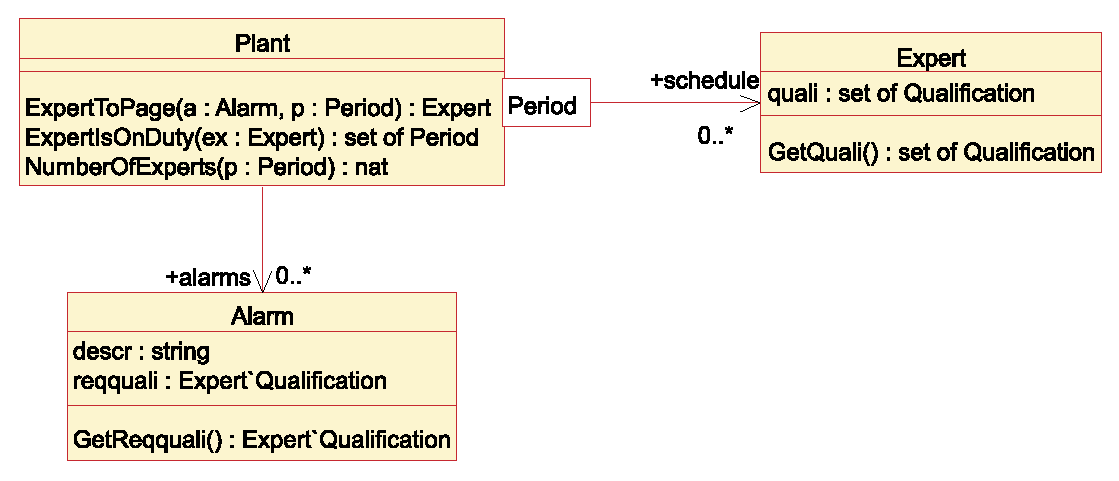
\includegraphics[width=5.5in]{updateddiagram}
\caption{The Updated UML Class Diagram.\label{fig:updateddiagram}}
\end{center}
\end{figure}

This gives a nice overview of the model, but has no detailed 
information about the requirements. The VDM++ model holds essential 
information for the implementation of the system. In this way 
the two models, or the two views of the same model, are complementary.

\section{Validating the VDM++ Model }

In the previous sections we have gone through the first steps 
of the construction of a model. We have seen how type checking 
facilities of \vdmtools\ can be used to check its internal consistency. 
Such facilities are useful but they do not allow us to detect 
all errors. In addition, validation can be used to get confidence 
that the model describes what the customer wanted, and to clarify 
what the customer thought was wanted.

Essentially there are two approaches to validating models which 
are based on systematic testing and rapid prototyping, respectively. 
Therefore \vdmtools\ supports the ability to validate models using 
conventional testing techniques and to execute models together 
with other code, e.g. a graphical front end. Hence, the interpreter 
of the VDM++ Toolbox is able to execute specifications symbolically, 
before they are implemented. During execution it automatically 
checks annotations, i.e. invariants and pre- and post-conditions. 
If some condition does not hold the user is notified with specific 
information about the violated condition and where the violation 
occurred. The stronger the conditions are and the more comprehensive 
the testing is, the higher the confidence in a model will be 
as a result of the validation. 

\subsection{Automated Validation Using Systematic Testing }

Models are tested in a traditional way, so we shall not go into 
the details of testing theory in this document. However, it is 
worth noting that the interpreter supports two modes of working. 
It is possible to test models interactively, where test expressions 
are given to the interpreter manually and evaluated immediately. 
The other mode is a batch mode, where the interpreter is executed 
automatically on a potentially large test suite. In this mode, 
it is possible to produce test coverage coloring of non-executed 
parts of a model as well as statistics about the execution.

In order to carry out testing it is often necessary to introduce 
operations for setting the values of the different instance variables, 
like the \texttt{SetReqquali} and \texttt{SetDescr} operations used above. Moreover, 
the operation \texttt{ExpertToPage} defined above cannot be executed in 
its current form. It is what we call an implicit operation because 
it does not have an operation body. However it is easy to turn 
the post-condition into a body and make the operation executable:

\begin{VDMgray}
  public
  ExpertToPage : Alarm * Period ==\texttt{>} Expert
  ExpertToPage(a, p) ==
    let ex in set schedule(p) be st
        a.GetReqquali() in set ex.GetQuali()
    in return ex
  pre a in set alarms and
      p in set dom schedule
  post let ex = RESULT in
         ex in set schedule(p) and
         a.GetReqquali() in set ex.GetQuali();
\end{VDMgray}


This uses a high-level VDM++ expression, called the let-be-such-that 
expression, which selects an arbitrary expert such that the predicate 
after ``be st'' holds, and then returns this expert.

The interpreter can execute commands like:

\small
\begin{alltt}
  create a1 := new Alarm()
  print a1.SetReqquali(\texttt{<}Mech\texttt{>})
  print a1.SetDescr("Mechanical fault")
\end{alltt}
\normalsize

The command \texttt{create} is used to make an instance of a class. The 
command \texttt{print} evaluates an expression, e.g. a method invocation 
as above. Each line can be typed to the interpreter manually 
or entire test scenarios can be set up in script files containing 
such commands. A script file is executed using the command script. 
Script files can call other script files as well. The following 
file is called test1, and is executed by typing \texttt{script test1}
in the interpreter window.

\small
\begin{alltt}
  init
  script testing/alarm1
  script testing/expert1
  create plant := new Plant()
  print plant.SetSchedule(\{plant.p1 {\textbar}-\texttt{>} \{ex1\}\})
  print plant.SetAlarms(\{a1\})
  print plant.ExpertIsOnDuty(ex1)
  print plant.ExpertToPage(a1,plant.p1) 
\end{alltt}
\normalsize

It calls two other scripts, the file \texttt{alarm1} which defines a new 
alarm object \texttt{a1}:

\small
\begin{alltt}
  create a1 := new Alarm()
  print a1.SetReqquali(\texttt{<}Mech\texttt{>})
  print a1.SetDescr("Mechanical fault")
\end{alltt}
\normalsize

And the file \texttt{expert1}, which defines a new expert object \texttt{ex1}:

\small
\begin{alltt}
  create ex1 := new Expert()
  print ex1.SetQuali(\{\texttt{<}Mech\texttt{>},\texttt{<}Bio\texttt{>}\})
\end{alltt}
\normalsize

The test script updates the schedule and set of alarms. At the 
same time, it checks invariants and other properties automatically.

\begin{figure}[H]
\begin{center}
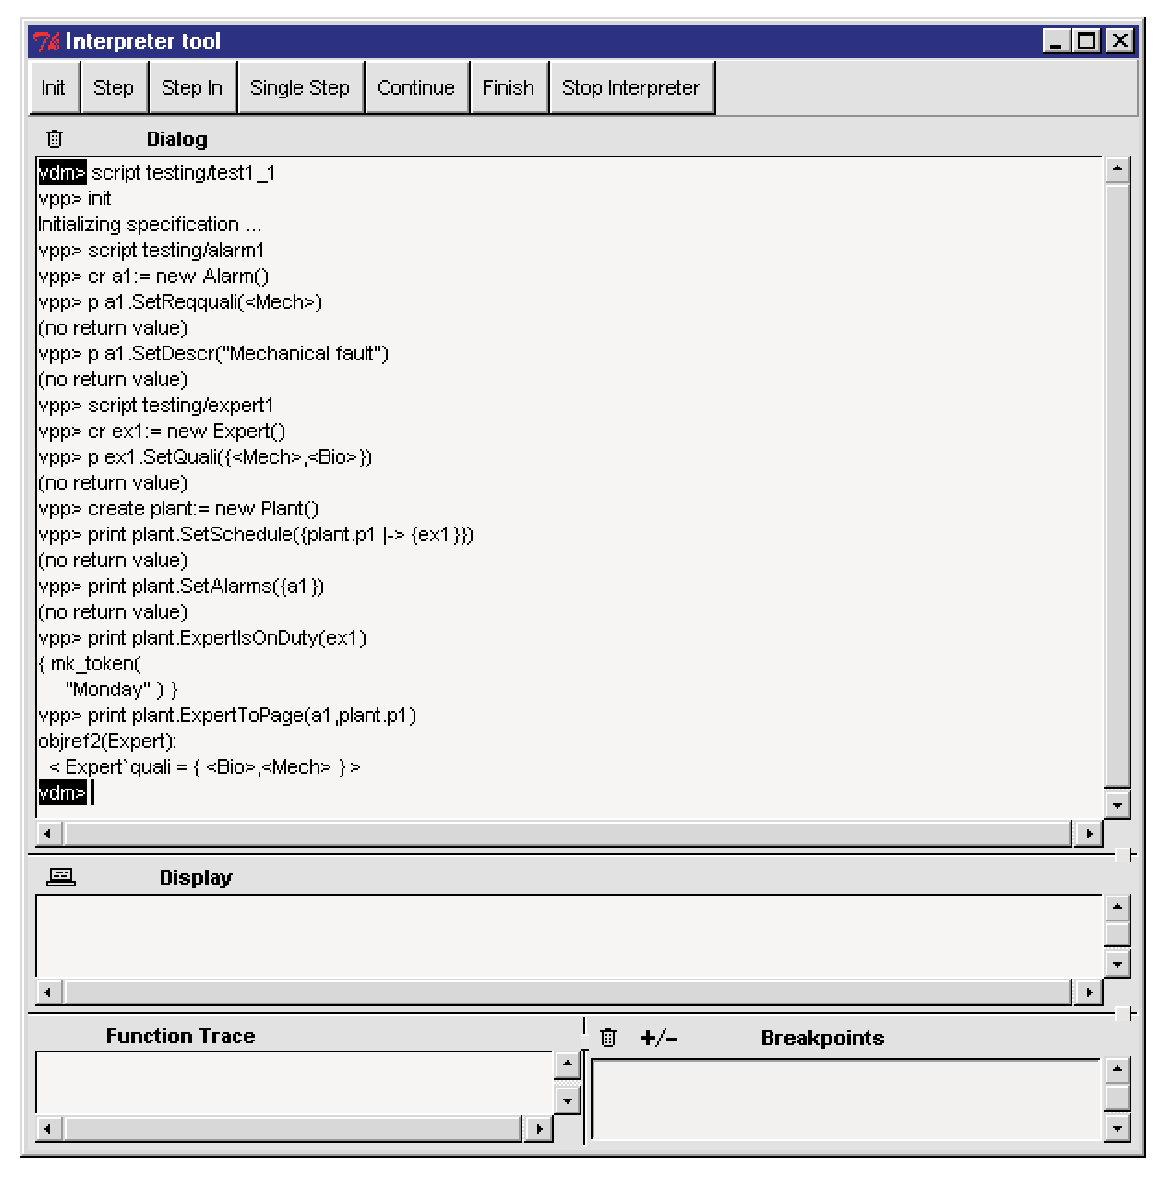
\includegraphics[width=5.546in]{firstscreendump}
\caption{Using the Interpreter.\label{fig:firstscreendump}}
\end{center}
\end{figure}

The identifier \texttt{p1} is a constant token value, defined in the class 
\texttt{Plant}. The version of the classes used during testing can be 
found in Appendix A. The figure above shows a screen dump of 
the Toolbox interpreter after executing the above \texttt{test1}
script as shown in Figure~\ref{fig:firstscreendump}.

The following test script executes \texttt{test1} above and then attempts 
to add a new alarm \texttt{a2} which requires the electrical qualification:

\small
\begin{alltt}
  script test1
  script alarm2
  print plant.SetAlarms(\{a1,a2\})
\end{alltt}
\normalsize

Here the script \texttt{alarm2} contains the following commands:

\small
\begin{alltt}
  create a2 := new Alarm()
  print a2.SetReqquali(\texttt{<}Elec\texttt{>})
  print a2.SetDescr("Electrical fault")
\end{alltt}
\normalsize

Note that the expert does not have the electrical qualification. 
Therefore this breaks the invariant as the screen dump 
from Figure~\ref{fig:secondscreendump} shows.

\begin{figure}[htpb]
\begin{center}
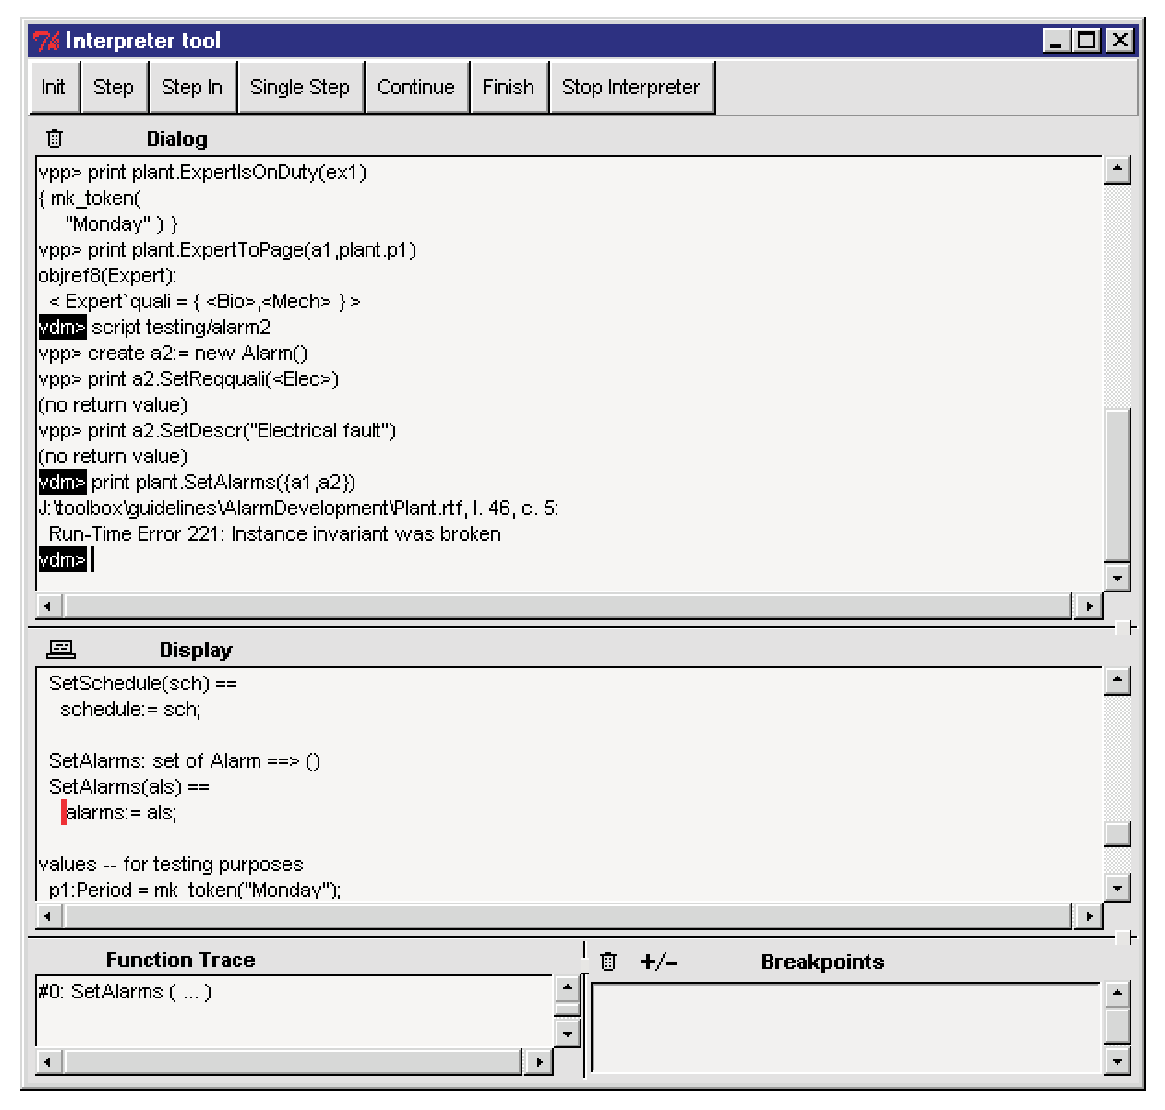
\includegraphics[width=5.546in]{secondscreendump}
\caption{Breaking an Invariant in the Interpreter.\label{fig:secondscreendump}}
\end{center}
\end{figure}

Note that the interpreter provides specific location information 
of the runtime error, and the error message says what is wrong. 
The display window shows in the specification source file where 
the problem was and the function trace gives the call stack, 
which in this case is only one deep. By clicking on the three 
dots in the function trace window, the argument of the listed 
operation call can be expanded.

The interpreter can also be used to debug specifications. It 
is possible to set breakpoints on functions 
and then interactively step through an execution and inspect 
variables in scope.

As part of the pretty-printing facility, it is possible to print 
test coverage information using colours in specifications.
%This requires that the Toolbox is used from the command line.
The VDM++ Toolbox is executed by typing vppde (VDM++ development 
environment) in a DOS or UNIX shell. This command takes various options, for example, 
``\texttt{-t}'' activates the type checker and ``\texttt{-i}'' activates the interpreter. 
Hence, the specification above is type checked by typing 

\small
\begin{alltt}
 vppde -t Plant.rtf Alarm.rtf Expert.rtf
\end{alltt}
\normalsize

The command line interpreter requires that we develop a so-called 
test argument file. This can contain a list of expressions to 
be evaluated by the interpreter. An example could be the following 
file which is called \texttt{test1.arg} and runs a version of the above 
test script:

\small
\begin{alltt}
 new Test1().run()
\end{alltt}
\normalsize

This uses a new class Test1:

\begin{VDMgray}
class Test1

instance variables
 a1 : Alarm;
 ex1 : Expert;
 plant : Plant;

operations
 public run: () ==\texttt{>} set of Plant\`{}Period * Expert
 run() == test1();

 test1: () ==\texttt{>} set of Plant\`{}Period * Expert
 test1() ==
   (alarm1();
    expert1();
    plant:= new Plant();
    plant.SetSchedule(\{plant.p1 {\textbar}-\texttt{>} \{ex1\}\});
    plant.SetAlarms(\{a1\});
    let periods = plant.ExpertIsOnDuty(ex1),
        expert = plant.ExpertToPage(a1,plant.p1)
    in 
      return mk\_(periods,expert));

 alarm1: () ==\texttt{>} ()
 alarm1() ==
   (a1:= new Alarm();
    a1.SetReqquali(\texttt{<}Mech\texttt{>});
    a1.SetDescr("Mechanical fault"));

 expert1: () ==\texttt{>} ()
 expert1() ==
   (ex1:= new Expert();
    ex1.SetQuali(\{\texttt{<}Mech\texttt{>},\texttt{<}Bio\texttt{>}\}))

end Test1
\end{VDMgray}


Then the following command is executed: 

\small
\begin{alltt}
  vppde -iDIPQ test1.arg Plant.rtf Alarm.rtf Expert.rtf Test1.rtf
\end{alltt}
\normalsize

While testing from the command line, the interpreter can collect 
test coverage information. This requires that we first produce 
a test coverage file as follows

\small
\begin{alltt}
  vppde -p -R vdm.tc Plant.rtf Alarm.rtf Expert.rtf Test1.rtf
\end{alltt}
\normalsize

and then execute a test case based on the argument file above

\small
\begin{alltt}
  vppde -iDIPQ -R vdm.tc test1.arg Plant.rtf
                         Alarm.rtf Expert.rtf Test1.rtf
\end{alltt}
\normalsize

The produced output file contains the expected result:

\small
\begin{alltt}
  mk\_( \{ mk\_token( 
   "Monday" ) \},
   objref4(Expert):
   \texttt{<} Expert\`{}quali = \{ \texttt{<}Bio\texttt{>},\texttt{<}Mech\texttt{>} \} \texttt{>} )
\end{alltt}
\normalsize

The resulting test coverage information is displayed in the pretty-printed 
specification in Appendix A.

Of course the vppde commands above can be called from batch or 
shell script files under Windows and Unix. This approach is recommended 
for systematic testing and is illustrated on a sorting example 
in the Toolbox User Manual \cite{UserManPP-SCSK}.

\subsection{Visual Validation Using Rapid Prototyping}

Testing is an excellent approach to validating a model and engineers 
master testing techniques well. However, the kind of relatively 
low-level testing introduced above is suitable mainly for engineers 
and less for customers, non-technical staff and management, who 
might not be familiar with VDM (or UML) and the details of a 
model. The VDM++ Toolbox provides an API to facilitate the need 
for presenting models to such an audience through a graphical 
front-end. The front-end can then work as graphical user interface 
to the model, so that customers can test the model directly via 
the GUI. An example of a simple front-end for the alarm example 
could look like in Figure~\ref{fig:javagui}

\begin{figure}[htbp]
\begin{center}
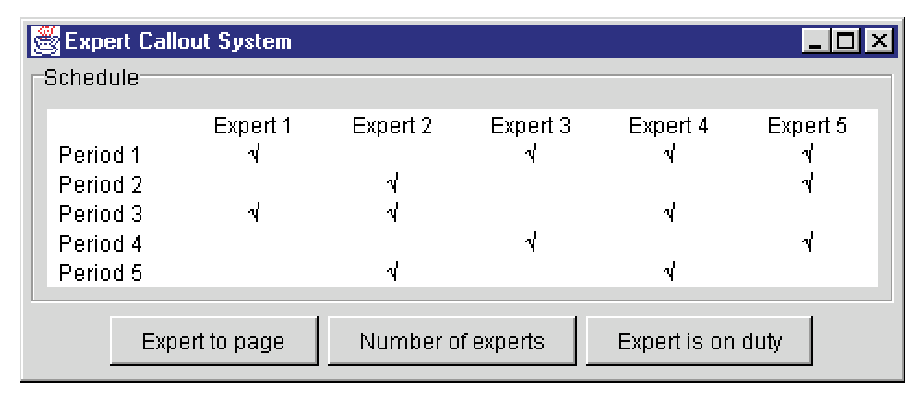
\includegraphics[width=4.999in]{javagui}
\caption{A Prototype GUI for the Alarm System.\label{fig:javagui}}
\end{center}
\end{figure}

Obviously better GUIs could be developed but this is not the 
essential point here, rather that users can easily use this to 
test the developer's understanding of the requirements of the 
system. In this way, the VDM++ model is used as an early prototype 
of the system. The front-end can be built using an engineer's 
favourite tool independent of VDM++. The one above was developed 
in Java/Swing.

The API can also be used to test models together with legacy 
systems, in fact, any other code independent of programming language, 
due to its general nature. This is because the API uses the Common 
Object Request Broker Architecture (CORBA), allowing communication 
with code written in any language for which an object request 
broker (ORB) exists. Currently free and commercial ORBs exist 
for all major languages. As CORBA is a network based architecture, 
this also means that multiple external clients located on a network 
can communicate with a single VDM++ Toolbox. Therefore this validation 
approach can also be used for distributed models.

\section{Code Generating the VDM++ Model}

Though the VDM++ model is an abstract model of the alarm system 
it is concrete enough to be code generated to Java or C++, compiled 
and run. The VDM++ Toolbox provides automatic code generators 
to accomplish this, which produce directly compilable, production 
quality code. Typically abstract models as the one above need 
more work before they can be code generated and delivered to 
a customer. Models for code generation are typically more design 
and implementation oriented, in particular, if there are strong 
efficiency requirements. However, even high-level expressions 
like the let-be-such-that expression introduced in the previous 
section can be code generated, compiled and run in Java and C++.

In addition to the obviously drastic reduction in the time to 
construct an implementation, automatic code generation offers 
a number of benefits. Principle amongst these is the strong correspondence 
between the abstract model and the generated code. This simplifies 
understanding of the code and its architectures. This also opens 
up the possibility of reusing test data originally used for testing 
the model. Of course it may be that the algorithm used in the 
generated code is inappropriate in a particular instance, so 
in this case it is possible to generate code skeletons which 
may then be hand implemented.

\section{Conclusions}

This document has presented some method guidelines for the construction 
of software models using VDM++. The methodology was applied to 
a simple example, an alarm system for a chemical plant. We would 
like to note that for brevity the model presented was abstract 
omitting many details. However, VDM++ can equally well support 
more concrete and substantially larger models e.g models corresponding 
to hundreds of pages of UML and thousands of lines of VDM++. 
The key to the approach described is the combination of UML and 
VDM++, so we conclude by summarising the complementary benefits 
of UML and VDM++.

\subsection{Who Should Use the Rose-VDM++ Link}

We believe that the following two groups of users can benefit 
from \vdmtools\ and its Rose-VDM++ Link:
\begin{enumerate}
\item
Those who apply or wish to apply a graphical modelling notation 
like UML in their software development process and want to improve 
and automate the reviewing and validation of models. Their motivation 
for doing this can be that their software is critical in some 
way or they want to reduce risk, and therefore they wish to obtain 
early and high confidence in their models by clarifying requirements 
and uncovering bugs as early as possible using the VDM technology.
\item
Those who apply or wish to apply a formal object-oriented specification 
language like VDM++ in their development process and want to 
get access to graphical visualisation capabilities for documentation 
purposes. 
\end{enumerate}


Both groups will probably use the link in more or less the same 
fashion. The first group may wish to do more modelling in UML 
while the second group will do more modelling in VDM++, but the 
round trip engineering capabilities of the link will be central 
to both groups. Hence, the users can benefit from starting the 
modelling at UML level because the graphical notation is better 
for obtaining an overview of the problem. Once, this model has 
reached a relatively fixed state it will be appropriate to translate 
the model to VDM++ and continue the analysis there, or switch 
back and forth between the two representations as desired. 

\subsection{Graphical Modelling in UML}

We believe that UML and Rose are more suitable for 
\begin{itemize}
\item
making the first sketches of an object-oriented model of a software 
system (in part supported by a piece of paper), 
\item
defining graphically visible aspects of a model such as class 
names, names of attributes and operations, signatures of operations 
and relations between classes (inheritance, associations, role 
names, etc.), 
\item
visual and efficient presentation of a model, e.g. through different 
diagram views, and
\item
documentation of abstract and high-level aspects of a software 
model.
\end{itemize}


An example of such a use of UML and Rose has been shown in this 
document.

\subsection{Analysing a Model using \vdmtools}

We believe that VDM++ and the \vdmtools are more suitable for

\begin{itemize}
\item
precise description of desired functionality, e.g. by formalising 
requirements properties as VDM++ invariants on instance variables 
and pre- and post-conditions on operations, 
\item
checking internal consistency of models using type checking, 
e.g. checking signatures of operations and types in declarations 
(attributes and associations in UML)
\item
defining and checking concrete aspects of models such as what 
operations should do, which would normally be expressed in natural 
language which is not checkable by tools, 
\item
gaining confidence in models through a systematic and repeatable 
reviewing process based on executing and testing models while 
consistency checking documented properties, and
\item
rapid prototyping where the model is executed together with a 
graphical front-end, or existing software for which a new component 
is being specified.
\end{itemize}


The beneficial use of the VDM technology to analyse a version 
of the SAFER model is described in the papers \cite{Agerholm&97c,Agerholm&99}. 
SAFER is a backpack module for astronauts to wear when they are 
outside a space shuttle to do a repair. Other papers on the VDM 
technology in the safety critical and security critical domains 
may also be of interest \cite{Agerholm&98a,Larsen&96a}.

\bibliographystyle{newalpha}

\bibliography{ifad}

\newpage
\appendix
\section{The UML and VDM++ Models}


This appendix lists the pretty-printed VDM++ classes of the model 
of the chemical plant example, plus a test class. For each class 
a test coverage table has been inserted by the \vdmtools\ pretty-printer. 
Non-executed parts of the model are coloured in red (or gray), 
see the operation NumberOfExperts in the class Plant.

The UML class diagram in Figure~\ref{fig:fulldiagram} gives an
overview of the model.

\begin{figure}[htbp]
\begin{center}
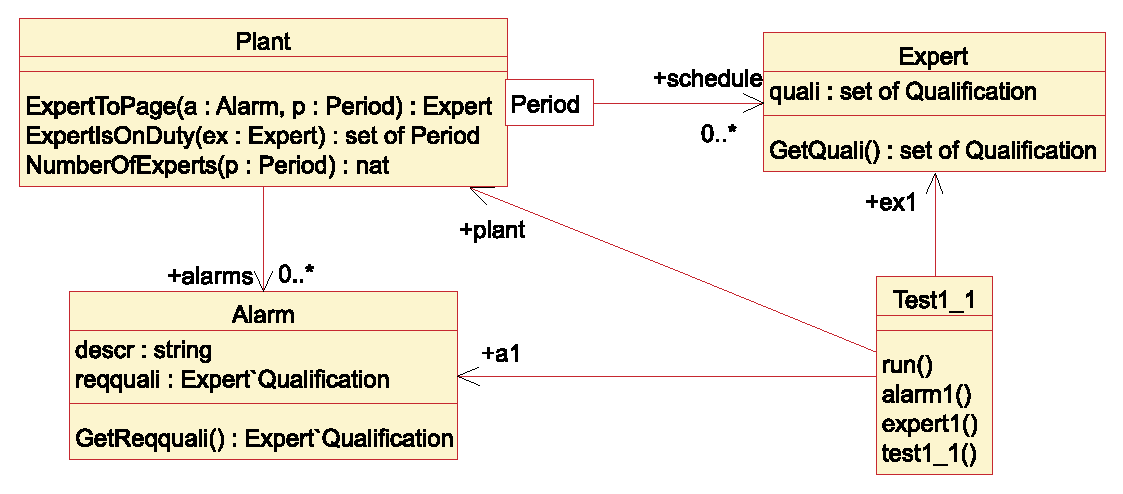
\includegraphics[width=5.967in]{fulldiagram}
\caption{The Full UML Class Diagram Model. \label{fig:fulldiagram}}
\end{center}
\end{figure}

\subsection{The Class Plant}

\begin{VDMgray}
\textbf{class} \textit{Plant}

\textbf{types}
 \textbf{public} \textit{Period} = \textbf{token};

\textbf{instance} \textbf{variables}
 \textit{alarms} : \textbf{set} \textbf{of} \textit{Alarm} := \{\};
 \textit{schedule} : \textbf{map} \textit{Period} \textbf{to} \textbf{set} \textbf{of} \textit{Expert} := \{{\textbar}-\texttt{>}\};
 \textbf{inv}
   \textbf{forall} \textit{p} \textbf{in set} \textbf{dom} \textit{schedule} \& \textit{schedule}(\textit{p}) \texttt{<}\texttt{>} \{\};
 \textbf{inv}
   \textbf{forall} \textit{a} \textbf{in set} \textit{alarms} \&
      \textbf{forall} \textit{p} \textbf{in set} \textbf{dom} \textit{schedule} \&
         \textbf{exists} \textit{ex} \textbf{in set} \textit{schedule}(\textit{p}) \&
            \textit{a}.\textit{GetReqquali}() \textbf{in set} \textit{ex}.\textit{GetQuali}();

\textbf{operations}
 \textbf{public}
 \textit{ExpertToPage} : \textit{Alarm} * \textit{Period} ==\texttt{>} \textit{Expert}
 \textit{ExpertToPage}(\textit{a}, \textit{p}) ==
   \textbf{let} \textit{ex} \textbf{in set} \textit{schedule}(\textit{p}) \textbf{be} \textbf{st}
       \textit{a}.\textit{GetReqquali}() \textbf{in set} \textit{ex}.\textit{GetQuali}()
   \textbf{in} \textbf{return} \textit{ex}
 \textbf{pre} \textit{a} \textbf{in set} \textit{alarms} \textbf{and}
     \textit{p} \textbf{in set} \textbf{dom} \textit{schedule}
 \textbf{post} \textbf{let} \textit{ex} = \textit{RESULT} \textbf{in}
       \textit{ex} \textbf{in set} \textit{schedule}(\textit{p}) \textbf{and}
       \textit{a}.\textit{GetReqquali}() \textbf{in set} \textit{ex}.\textit{GetQuali}();

 \textbf{public}
 \textit{ExpertIsOnDuty} : \textit{Expert} ==\texttt{>} \textbf{set} \textbf{of} \textit{Period}
 \textit{ExpertIsOnDuty}(\textit{ex}) ==
   \textbf{return} \{\textit{p} {\textbar} \textit{p} \textbf{in set} \textbf{dom} \textit{schedule} 
             \& \textit{ex} \textbf{in set} \textit{schedule}(\textit{p})\};

 \textbf{public}
 \textit{NumberOfExperts} : \textit{Period} ==\texttt{>} \textbf{nat}
 \textit{NumberOfExperts}(\textit{p}) ==
  {\color{color6} \textbf{return}} {\color{color6} \textbf{card}} {\color{color6} \textit{schedule}}{\color{color6} (}{\color{color6} \textit{p}}{\color{color6} )
} \textbf{pre} {\color{color6} \textit{p}} {\color{color6} \textbf{in set}} {\color{color6} \textbf{dom}} {\color{color6} \textit{schedule}};
\end{VDMgray}

\begin{VDMgray}
 \textbf{public}
 \textit{SetSchedule}: \textbf{map} \textit{Period} \textbf{to} \textbf{set} \textbf{of} \textit{Expert} ==\texttt{>} ()
 \textit{SetSchedule}(\textit{sch}) ==
   \textit{schedule}:= \textit{sch};

 \textbf{public}
 \textit{SetAlarms}: \textbf{set} \textbf{of} \textit{Alarm} ==\texttt{>} ()
 \textit{SetAlarms}(\textit{als}) ==
   \textit{alarms}:= \textit{als};

\textbf{values} -- for testing purposes
  \textbf{public} \textit{p1}:\textit{Period} = \textbf{mk\_token}("Monday");
  \textbf{public} \textit{p2}:\textit{Period} = \textbf{mk\_token}("Tuesday");
  \textbf{public} \textit{p3}:\textit{Period} = \textbf{mk\_token}("Wednesday");
  \textbf{public} \textit{p4}:\textit{Period} = \textbf{mk\_token}("Thursday");
  \textbf{public} \textit{p5}:\textit{Period} = \textbf{mk\_token}("Friday");

\textbf{end} \textit{Plant}
\end{VDMgray}


\begin{longtable}{lll}
\hline
\endhead
\hline
\endfoot
\hline
\multicolumn{1}{|p{3.086in}|}
{\raggedright
\textbf{\textit{name}}} & 
\multicolumn{1}{p{0.660in}|}
{\raggedright
\textbf{\textit{\#calls}}} & 
\multicolumn{1}{p{0.754in}|}
{\raggedright
\textbf{\textit{coverage}}}
\\ \cline{1-1}\cline{2-2}\cline{3-3}
\multicolumn{1}{|p{3.086in}|}
{\raggedright
Plant\`{}ExpertIsOnDuty } & 
\multicolumn{1}{p{0.660in}|}
{\raggedright
  1 } & 
\multicolumn{1}{p{0.754in}|}
{\raggedright
100\%}
\\ \cline{1-1}\cline{2-2}\cline{3-3}
\multicolumn{1}{|p{3.086in}|}
{\raggedright
Plant\`{}ExpertToPage } & 
\multicolumn{1}{p{0.660in}|}
{\raggedright
  1 } & 
\multicolumn{1}{p{0.754in}|}
{\raggedright
100\%}
\\ \cline{1-1}\cline{2-2}\cline{3-3}
\multicolumn{1}{|p{3.086in}|}
{\raggedright
Plant\`{}NumberOfExperts } & 
\multicolumn{1}{p{0.660in}|}
{\raggedright
  0 } & 
\multicolumn{1}{p{0.754in}|}
{\raggedright
0\%}
\\ \cline{1-1}\cline{2-2}\cline{3-3}
\multicolumn{1}{|p{3.086in}|}
{\raggedright
Plant\`{}SetAlarms } & 
\multicolumn{1}{p{0.660in}|}
{\raggedright
  1 } & 
\multicolumn{1}{p{0.754in}|}
{\raggedright
100\%}
\\ \cline{1-1}\cline{2-2}\cline{3-3}
\multicolumn{1}{|p{3.086in}|}
{\raggedright
Plant\`{}SetSchedule } & 
\multicolumn{1}{p{0.660in}|}
{\raggedright
  1 } & 
\multicolumn{1}{p{0.754in}|}
{\raggedright
100\%}
\\ \cline{1-1}\cline{2-2}\cline{3-3}
\multicolumn{1}{|p{3.086in}|}
{\raggedright
\textbf{\textit{total}}} & 
\multicolumn{1}{p{0.660in}|}
{\raggedright
} & 
\multicolumn{1}{p{0.754in}|}
{\raggedright
\textbf{\textit{84\% }}} \\
\hline
\end{longtable}

\subsection{The Class Expert}

\begin{VDMgray}
\textbf{class} \textit{Expert}

\textbf{types}
 \textbf{public} \textit{Qualification} = \texttt{<}Mech\texttt{>} {\textbar} \texttt{<}Chem\texttt{>} {\textbar} \texttt{<}Bio\texttt{>} {\textbar} \texttt{<}Elec\texttt{>};

\textbf{instance} \textbf{variables}
 \textit{quali} : \textbf{set} \textbf{of} \textit{Qualification};

\textbf{operations}
 \textbf{public}
 \textit{GetQuali}: () ==\texttt{>} \textbf{set} \textbf{of} \textit{Qualification}
 \textit{GetQuali}() == \textbf{return} \textit{quali};

 \textbf{public}
 \textit{SetQuali}: \textbf{set} \textbf{of} \textit{Qualification} ==\texttt{>} ()
 \textit{SetQuali}(\textit{qs}) ==
   \textit{quali}:= \textit{qs};

\textbf{end} \textit{Expert}
\end{VDMgray}


\begin{longtable}{lll}
\hline
\endhead
\hline
\endfoot
\hline
\multicolumn{1}{|p{3.086in}|}
{\raggedright
\textbf{\textit{name}}} & 
\multicolumn{1}{p{0.660in}|}
{\raggedright
\textbf{\textit{\#calls}}} & 
\multicolumn{1}{p{0.754in}|}
{\raggedright
\textbf{\textit{coverage}}}
\\ \cline{1-1}\cline{2-2}\cline{3-3}
\multicolumn{1}{|p{3.086in}|}
{\raggedright
Expert\`{}GetQuali } & 
\multicolumn{1}{p{0.660in}|}
{\raggedright
  3 } & 
\multicolumn{1}{p{0.754in}|}
{\raggedright
100\%}
\\ \cline{1-1}\cline{2-2}\cline{3-3}
\multicolumn{1}{|p{3.086in}|}
{\raggedright
Expert\`{}SetQuali } & 
\multicolumn{1}{p{0.660in}|}
{\raggedright
  1 } & 
\multicolumn{1}{p{0.754in}|}
{\raggedright
100\%}
\\ \cline{1-1}\cline{2-2}\cline{3-3}
\multicolumn{1}{|p{3.086in}|}
{\raggedright
\textbf{\textit{total}}} & 
\multicolumn{1}{p{0.660in}|}
{\raggedright
} & 
\multicolumn{1}{p{0.754in}|}
{\raggedright
\textbf{\textit{100\% }}}\\
\hline
\end{longtable}

\subsection{The Class Test1}


\begin{VDMgray}
\textbf{class} \textit{Test1}

\textbf{instance} \textbf{variables}
 \textit{a1} : \textit{Alarm};
 \textit{ex1} : \textit{Expert};
 \textit{plant} : \textit{Plant};

\textbf{operations}
 \textbf{public}
 \textit{run}: () ==\texttt{>} \textbf{set} \textbf{of} \textit{Plant}\`{}\textit{Period} * \textit{Expert}
 \textit{run}() == \textit{test1}();

 \textbf{public}
 \textit{test1}: () ==\texttt{>} \textbf{set} \textbf{of} \textit{Plant}\`{}\textit{Period} * \textit{Expert}
 \textit{test1}() ==
   (\textit{alarm1}();
    \textit{expert1}();
    \textit{plant}:= \textbf{new} \textit{Plant}();
    \textit{plant}.\textit{SetSchedule}(\{\textit{plant}.\textit{p1} {\textbar}-\texttt{>} \{\textit{ex1}\}\});
    \textit{plant}.\textit{SetAlarms}(\{\textit{a1}\});
    \textbf{let} \textit{periods} = \textit{plant}.\textit{ExpertIsOnDuty}(\textit{ex1}),
        \textit{expert} = \textit{plant}.\textit{ExpertToPage}(\textit{a1},\textit{plant}.\textit{p1})
    \textbf{in}
      \textbf{return} \textbf{mk\_}(\textit{periods},\textit{expert})
  );

 \textbf{public}
 \textit{alarm1}: () ==\texttt{>} ()
 \textit{alarm1}() ==
   (\textit{a1}:= \textbf{new} \textit{Alarm}();
    \textit{a1}.\textit{SetReqquali}(\texttt{<}Mech\texttt{>});
    \textit{a1}.\textit{SetDescr}("Mechanical fault"));

 \textbf{public}
 \textit{expert1}: () ==\texttt{>} ()
 \textit{expert1}() ==
   (\textit{ex1}:= \textbf{new} \textit{Expert}();
    \textit{ex1}.\textit{SetQuali}(\{\texttt{<}Mech\texttt{>},\texttt{<}Bio\texttt{>}\}))

\textbf{end} \textit{Test1}
\end{VDMgray}


\begin{longtable}{lll}
\hline
\endhead
\hline
\endfoot
\hline
\multicolumn{1}{|p{3.086in}|}
{\raggedright
\textbf{\textit{name}}} & 
\multicolumn{1}{p{0.660in}|}
{\raggedright
\textbf{\textit{\#calls}}} & 
\multicolumn{1}{p{0.754in}|}
{\raggedright
\textbf{\textit{coverage}}}
\\ \cline{1-1}\cline{2-2}\cline{3-3}
\multicolumn{1}{|p{3.086in}|}
{\raggedright
Test1\`{}alarm1 } & 
\multicolumn{1}{p{0.660in}|}
{\raggedright
  1 } & 
\multicolumn{1}{p{0.754in}|}
{\raggedright
100\%}
\\ \cline{1-1}\cline{2-2}\cline{3-3}
\multicolumn{1}{|p{3.086in}|}
{\raggedright
Test1\`{}expert1 } & 
\multicolumn{1}{p{0.660in}|}
{\raggedright
  1 } & 
\multicolumn{1}{p{0.754in}|}
{\raggedright
100\%}
\\ \cline{1-1}\cline{2-2}\cline{3-3}
\multicolumn{1}{|p{3.086in}|}
{\raggedright
Test1\`{}run } & 
\multicolumn{1}{p{0.660in}|}
{\raggedright
  1 } & 
\multicolumn{1}{p{0.754in}|}
{\raggedright
100\%}
\\ \cline{1-1}\cline{2-2}\cline{3-3}
\multicolumn{1}{|p{3.086in}|}
{\raggedright
Test1\`{}test1 } & 
\multicolumn{1}{p{0.660in}|}
{\raggedright
  1 } & 
\multicolumn{1}{p{0.754in}|}
{\raggedright
100\%}
\\ \cline{1-1}\cline{2-2}\cline{3-3}
\multicolumn{1}{|p{3.086in}|}
{\raggedright
\textbf{\textit{total}}} & 
\multicolumn{1}{p{0.660in}|}
{\raggedright
} & 
\multicolumn{1}{p{0.754in}|}
{\raggedright
\textbf{\textit{100\% }}}\\
\hline
\end{longtable}

  

\end{document}
